

These strong inferences are puzzling when examined next to the prevalence required for a generic to be true. 
As we saw in Expt.~1, generics can be true for a range of prevalence levels. 
This phenomenon clearly distinguishes generic statements from quantified statements.
``All lorches have purple feathers.'' is true only when 100\% of lorches have purple feathers. 
Similarly, upon hearing such an utterance, one is likely to infer that 100\% of lorches have purple feathers.  
This symmetric relationship holds with the quantifier ``most'', but generic utterances don't behave in this way \cite{Cimpian2010}.
Generic statements are judged true for a wide range of prevalence levels, but upon hearing a generic utterance, participants were wont to infer that \emph{almost all} of the category have the property. 
The implications of generic statements go far beyond the evidence needed to accept them as valid utterances.

The strength of the inference also depends on the property in question.
\citeA{Cimpian2010} observed that predicating bare plurals with accidental properties (e.g. ``Lorches have muddy feathers.'') significantly reduced participants' judgments about the implied prevalence of these statements.

Expt.~2 attempted to replicate, extend and explain the findings of \citeA{Cimpian2010}: that there is an asymmetry between truth conditions and implied prevalence of the generic and that this asymmetry is sensitive to the type of property predicated. 
In Expt.~2a, we measure participants' beliefs about the distribution of these types of properties using a paradigm generalized from Expt.~1a. 
In Expt.~2b, we replicate and extend \citeauthor{Cimpian2010}'s findings to different classes of properties for which the prevalence priors differed. 
We show that the language understanding model predicts this asymmetry between truth conditions and implications, and that this asymmetry can be manipulated by differences in the prevalence distributions between properties.








The largest deviations occur for the items ``Robins carry malaria.'' and ``Sharks have manes.''. 
Neither of these is true, and participants judge them to be as such.
The model predictions these are bad but better than items such as ``Leopards have wings.'' 
This difference is likely driven by greater uncertainty about the prevalence of the properties ``carries malaria'' and ``has manes'' as compared with ``has wings''.
``Carries malaria'' and ``has manes'' produced a more uncertain distribution of responses \red{(cite concentration parameters here..)} compared with ``has wings.''








We use these estimates as the prevalence of property for the target category in the model. 





 
 
 
 
 
 
 
 
 
 
 
 
 
 
 
 
 
 
 
 
 
 
 
 
 
 
In the experiments that follow, we explore the predictions of the $S_2$ model by comparing them to participant acceptability judgments of natural cases of generic utterances. 
We also verify the predictions of the $L_1$ model by comparing them to participants' interpretations of novel generic sentences.
These predictions are borne out by first eliciting the prior distribution on prevalence.
 

In a similar way, we posit a simple, scalar semantics for generics in which they express that the probability of the property given the category-----i.e. the property's \emph{prevalence}-----is above a threshold (cf. \citeA{Cohen1999}). We treat this threshold as unknown property of the language and thus, as a variable that must be reasoned about in context. 

It might seem paradoxical that vague language should get so much usage. 
Shouldn't speakers want to express their ideas as clearly as possible?
Language evolutionary pressures suggest that, to the contrary, such underspecification is in fact useful, given that there is some context through which the uncertainty can be resolved \cite{Piantadosi2012}.
In this work, context takes the shape of a listener and speaker's shared beliefs (i.e. common ground) about the property in question. This, coupled with 
standard inferences from conversational pragmatics, allows the listener to figure out the meaning of the otherwise vague utterance.
We extend the \emph{Rational Speech-Acts} (RSA) framework \cite{Frank2012,Goodman2013} to consider how a speaker determines what generics are acceptable to produce and how a listener might interpret generics differently depending on her belief's about the property in question. 
This formalism gives a new, computational perspective on how ideas are conveyed and how beliefs play a central role in understanding language.

\subsection{The phenomena}

One important test for a theory of generic meaning is that it captures the intuition shared by language users about the truth of certain generic sentences. To test the predictions of this model, we must first measure participants' prior expectations about the prevalence of the properties in question. Critically, however, we must measure not only prior expectations about the prevalence of the property for the category \emph{alone} but the distribution of expectations across categories (i.e. not only the probability of laying eggs for a robin, but also the probability of laying eggs for a cow and other animal species).  
We show how prevalence within the category alone is insufficient to explain generic acceptability, but a model that reasons pragmatically about the distribution over prevalence is sufficient to explain the variability in truth judgments.

Generic statements are not only puzzling because of their variable truth conditions, but also because of how they are interpreted. \citeA{Gelman2002} found that listeners  interpret novel facts about animals in the form of generics (e.g. ``Bears like to eat ants.'') as applying to nearly all of the category. Interpretations of bare plurals of novel animals with accidental properties (e.g. ``Morseths have wet fur.'') were found to be much weaker \cite{Cimpian2010}. These differences in interpretation are thought to be a result of different beliefs about the properties in question. This intuition is readily formalized in our language understanding model. Beliefs about properties are measured in independent experiments to serve as a foundation for the model's predictions. 
We compare our model's predictions to experiments examining the acceptability of naturalistic generics and interpretations of generics about novel categories.
\section{Experiment 1: Truth value judgments}

The lifted-threshold RSA model specified in Eq.~\ref{eq:S2} predicts probabilities of producing a generic given a prior distribution on the prevalence of the property. 
In Expt.~1a, we measure the distribution on prevalence of certain target properties by asking participants about the percentage of a kind with the property \footnote{So as to not bias the measurement in favor of a small number of stipulated animal categories, we ask participants to generate their own animal categories.}. 
In Expt.~1b, we measure the acceptability of a number of generic statements about the properties measured in Expt. 1a. 
We show how the prevalence within a property alone is insufficient to explain the diversity of truth judgments of these generics, but how a model of a pragmatic speaker who considers the distribution on prevalence can explain this wide range of truth judgments.



\section{Experiment 2: Generics carry strong implications}
\subsection{Experiment 2a: \emph{Prior elicitation for properties of novel animals}}

In this experiment, we measured participants' beliefs about the distribution of the prevalence of certain properties within- and across- animal kinds. 
We expanded the stimulus set from \citeA{Cimpian2010} which consisted of novel animal categories (e.g. glippets) and various properties (e.g. have orange legs; have broken legs).


\subsubsection{Participants}

We recruited 40 participants over Amazon's crowd-sourcing platform Mechanical Turk (MTurk).  Participants were restricted to those with US IP addresses and with at least a 95\% MTurk work approval rating. All participants were native English speakers. The experiment took about 5-7 minutes and participants were compensated \$0.75.

\subsubsection{Procedure and materials}

In Expt.~1a, participants filled out a table with rows corresponding to different animal kinds and columns corresponding to different properties. 
Pilot testing suggested this was a pragmatically strange setup for this paradigm: answering ``What percentage of lorches have purple feathers?'', when participants knew nothing about lorches was difficult.
We took advantage of the latent structure in the task, described in Section \ref{sec:bda1}, and used a Bayesian statistical model to infer the underlying distribution. 
We then used these distributions in our language model to make predictions about the implications of generic sentences.

Participants were asked about the prevalence across categories by asking them the likelihood of there existing a K that has F, where K was a novel animal category and F was a property (e.g. ``how likely is it that there is a lorch that is female?''). 
Prevalence within categories was measured by asking participants about the percentage of Ks that have Fs, given that at least one does.
Participants responded using slider bars that ranged from ``unlikely'' to ``likely'', and ``0\%'' to ``100\%'', respectively.
Complete instructions shown to participants are in Appendix \ref{sec:prior2instruct}. 

Materials---novel animal names and familiar properties---built upon those from \citeA{Cimpian2010}. 
Classic work in generalization suggested to us that there may be differences in the implications of generic statements of different types of biological properties \cite{Nisbett1983}. 
We expanded the stimulus set to include four different types of properties: biological parts (e.g. ``feathers''), colored parts (e.g. ``purple feathers''), vague parts (e.g. ``smooth feathers''), and accidental parts (e.g. ``broken feathers''). 
Pilot testing revealed a lot of variability across items in the accidental properties relative to the other types of properties. 
To test the quantitative predictive power of the generic interpretation model, we used twice as many exemplars of accidental properties, with the aim to make a ``common accidental'' and a ``rare accidental'' class of properties. 
We used 8 exemplars of each of the three non-accidental properties (``parts'', ``colored parts'', ``vague parts'') and 16 exemplars of accidental properties.
Materials are in Appendix \ref{sec:materials2}.

\subsubsection{Bayesian data analysis}
\ref{sec:bda2}
In order to recover single belief distributions representing prevalence both within- and across- categories (analogous to those elicited in Expt.~1a and shown in Figure \ref{fig:priors1a}), we built a simple Bayesian statistical model of the task questions and their relation to the desired distribution. 

Participants' responses to each question (slider bar values) were assumed to be samples from Beta distributions with unknown means and concentrations. 
The responses to the questions ($d_{across}, d_{within}$) were used to estimate the parameters of the distributions of prevalence across- and within- categories, separately. 
\begin{align*}
d_{across} \sim \text{Beta}(\gamma_{across}, \delta_{across}) \\
d_{within} \sim \text{Beta}(\gamma_{within}, \delta_{within}) 
\end{align*}
The parameters $\gamma$ and $\delta$ correspond to the mean and variance (formally, the concentration), respectively, of prevalence for each of the across- and within- distributions.
As in our other models, we assume some global proportion of noise in the experimental data $\phi$. 
We put identical, uninformative priors on these parameters:
\begin{align*}
\phi & \sim \text{Uniform}(0,1) \\
\gamma & \sim \text{Uniform}(0,1) \\
\delta & \sim \text{Uniform}(0,20) 
\end{align*}
To construct single prevalence distributions reflecting both the within- and across- category prevalence (as we have for Expt.~1a), we assume that the distribution is a mixture of categories that have the property and categories that don't have the property\footnote{This is similar in spirit to Hurdle Models of count data used in clinical trials where the observed proportion of zeros is greater than one would expect from classical models of count data like the Poisson model.}. Whether or not a category has a property ($h$) is driven by the prevalence across categories ($\theta_{across}$).
%
\begin{align*}
\theta_{across} & \sim \text{Beta}(\gamma_{across}, \delta_{across}) \\ 
h & \sim \text{Bernoulli}(\theta_{across}) \\
x & \sim \begin{cases} 
		\text{Beta}(\gamma_{within}, \delta_{within}) &\mbox{if } h = 1 \\ 
				0 & \mbox{if } h=0. 
				\end{cases} 
\end{align*}
%
Marginal posterior distributions for $x$ were estimated using the Metropolis-Hastings algorithm in the probabilistic programming language WebPPL \cite{dippl}. Inference was completed by taking 50,000 samples using the Metropolis-Hastings algorithm.

\subsubsection{Results}

Our focus for this experiment is to see if the distributions on prevalence differ between the different types of properties.
We analyzed the data first by item in order to split the accidental properties into two categories: common accidental properties (e.g. wet fur) and rare accidental properties (e.g. broken legs). We then ran the model again analyzing the data by type of property.

Figure \ref{fig:prior2} (left) shows the posterior predictive distributions for prevalence $x$ for 5 different types of properties
.Figure \ref{fig:prior2} (right) shows the region of interest of these distributions by removing the mass at 0. 
These distributions form the prevalence priors used in the language understanding model for Expt.~2b. 
With the exception of the body part category, properties are mostly likely to be absent from the category (Figure \ref{fig:prior2} left; modes of distributions are at 0).
If the property is present in the category, the most likely prevalence for biological properties (``part'', ``color part'', and ``vague part'') is 100\% (Figure \ref{fig:prior2} right; modes of blue, green, and red distributions are at 1).
This is not the case with the prevalence priors for accidental properties, for which lower values are more likely (Figure \ref{fig:prior2} right; modes of orange and purples distributions are at some low prevalence).


\begin{figure}
\centering
    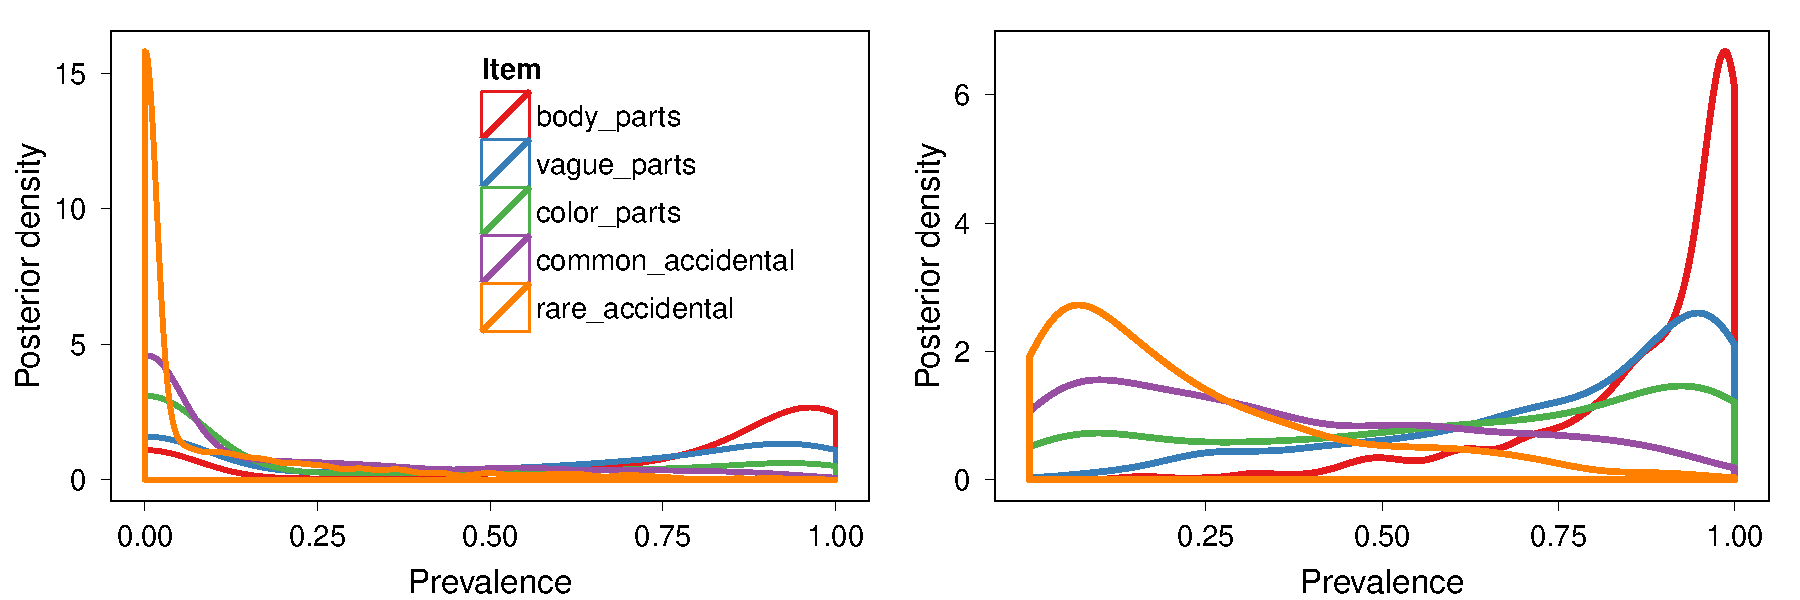
\includegraphics[width=\columnwidth]{prior2_prevalenceprior-50k.pdf}
    \caption{Prevalence priors inferred from the prior elicitation experiment  (Expt.~1a). Right plot shows all non-zero probability mass. This corresponds to the expected within-category prevalence. Different types of properties have different likely prevalence values.}
  \label{fig:prior2}
\end{figure}

\subsection{Experiment 2b: mistmaches between \emph{truth conditions} and \emph{implications}}

\citeauthor{Cimpian2010} observed that generic statements of novel kinds with biological properties (e.g. ``Glippets have yellow fur'') show an asymmetry between the conditions by which the generic is true (``\emph{truth conditions}'') and the prevalence implied by the generic (``\emph{implied prevalence}''). 
Generic sentences were endorsed for a wide-range of prevalence levels (e.g. when ``30\% of glippets have yellow fur.''), resulting in intermediate average truth conditions. 
Upon hearing a generic, listeners inferred that the property was widespread (e.g. almost all glippets have yellow fur).
This mismatch between \emph{truth conditions} and \emph{implied prevalence} was significantly reduced for generics of properties plausibly construed as accidental (e.g. ``Glippets have wet fur.'').

In this experiment,  we replicate these findings and extend them to reveal even more variability in the mismatch between \emph{truth conditions} and \emph{implied prevalence} using the types of properties from Expt.~2a.
We also show how the prevalence-based model predicts the variability in the mismatch with strong quantitative accuracy.


\subsubsection{Participants}

We recruited 80 participants over Amazon's crowd-sourcing platform Mechanical Turk (MTurk).  
Participants were restricted to those with US IP addresses and with at least a 95\% MTurk work approval rating. 
All participants were native English speakers. 
The experiment took about 5 minutes and participants were compensated \$0.60.

\subsubsection{Procedure and materials}

In order to get participants motivated to reason about novel animals, they were told they were the resident zoologist of a team of scientists that recently discovered an island with many new animals; their task was to provide their expert opinion on questions about these animals\footnote{The experiment in full can be viewed at \url{http://stanford.edu/~mtessler/generics/experiments/asymmetry/asymmetry-2.html}}. 
We recruited 40 participants for the \emph{truth conditions} task and 40 participants for the \emph{implied prevalence task}. 

Following \citeauthor{Cimpian2010}'s paradigm, in the \emph{truth conditions} task, participants were given an evidence statement consisting of the percentage of a novel animal category that had a property (e.g.~``30\% of glippets have yellow fur''). 
Participants were asked if they agreed or disagreed with the associated generic statement (i.e.~``Glippets have yellow fur.'').
Prevalence varied between 10, 30, 50, 70, and 90\%.
The experiment consisted of 25 trials: 5 trials for each of 5 types of properties measured in Expt.~2a (part, color part, vague part, common accidental, rare accidental). 
Each prevalence level appeared once for each property type (5 prevalence levels x 5 property types). 

Participants in the \emph{implied prevalence} task were supplied with the generic (e.g. ``Glippets have yellow fur.'') and asked to judge prevalence: ``What percentage of glippets do you think have yellow fur?''. Participants saw 25 trials: 5 for each of 5 property types.
The original study by \citeauthor{Cimpian2010} found a difference in the implied prevalence between ``color parts'' (e.g. yellow fur) and accidental properties (e.g. wet fur).
The prevalence priors inferred from Expt.~2a suggest that generic interpretation should be even more variable than simply strong vs. weak.
For this reason, we included three types of biological properties: parts (e.g. fur), color--part pairs (e.g. yellow fur) and gradable adjective--part pairs (e.g. curly fur). 
We also coded the accidental properties from Expt.~2a as either ``common'' or ``rare'' using a by-item median split.

 
Most of the materials we used were from \citeauthor{Cimpian2010}. 
The materials used were 30 novel animal categories (e.g. lorches, morseths, blins) each paired with a unique property. 
Biological properties were made by pairing a color with a body-part (e.g. purple feathers, orange tails). 
Accidental properties used the same set of body-parts but modified it with an adjective describing an accidental or disease state (e.g. broken legs, wet fur). 
Each participant saw a random subset of 10 unique animal-property pairs for each type of property (biological and accidental). 
Table \ref{tab:sampleTrial} shows an example trial for each of the property types and tasks.


\begin{table}[h]
\begin{tabular}{| l |  l | l | l |}
\hline
           &             & Truth conditions                                                                                                    & Implied prevalence                                            \\
           \hline \hline
Biological &             &                                                                                                                     &                                                               \\
\hline
           & Information & xx\% of lorches have purple feathers.                                                                               & Lorches have purple feathers.                                 \\
\hline
           & Question    & \begin{tabular}[c]{@{}l@{}}Is the following sentence true or false?\\ \\ Lorches have purple feathers.\end{tabular} & \begin{tabular}[c]{@{}l@{}}What percentage of lorches \\do you think have purple feathers?\end{tabular} \\
           \hline \hline
Accidental &             &                                                                                                                     &                                                               \\
\hline
           & Information & xx\% of lorches have muddy feathers.                                                                                & Lorches have muddy feathers.                                  \\
\hline
           & Question    & \begin{tabular}[c]{@{}l@{}}Is the following sentence true or false?\\ \\ Lorches have muddy feathers.\end{tabular}  & \begin{tabular}[c]{@{}l@{}}What percentage of lorches \\ do you think have muddy feathers?\end{tabular} \\
\hline
\end{tabular}
\caption{Sample item from Experiment 2}
\label{tab:sampleTrial}

\end{table}

\subsubsection{Results}



Results are shown in Figure~\ref{fig:exp2b} (Left). 
\subsubsection{Lifted-threshold model predictions}

In Expt.~1, the acceptability of the generic was modeled as a speaker (Eq.~\ref{eq:S2}) reasoning about whether or not to produce the generic given some known prevalence. 
We use the same model to make predictions for the \emph{truth conditions} data.
The \emph{implied prevalence} task is slightly different: Here, the participant hears a generic and is asked to infer the likely prevalence of the property. 
This is the model of the listener in Eq.~\ref{eq:L1}. 
We use this model to predict the data from the implied prevalence task.

Each of these models has a parameter governing the optimality of the hypothetical speaker in Eq.~\ref{eq:S1}. 
Since the supports of the distributions produced by the two models are different ($S_2$ returns a distribution over ``agree'' and ``disagree'', whereas $L_1$ generates a distribution prevalence levels), there is no reason to believe the speaker optimality parameters would be the same for the two models. 
Hence, we put independent prior distributions over the two parameters: $\lambda_{\text{truth conditions}}, \lambda_{\text{implied prevalence}} \sim \text{Uniform}(0, 20)$.

We model the observed data as being generated by a mixture of our generics model and a model of random guessing behavior. 
Modeling random guessing explicitly is important for recovering reliable estimates of the parameters of the model, which would otherwise be contaminated by this data \cite{LW2014}.
We put an uniformative prior over this mixture parameter $\phi \sim \text{Uniform}(0,1)$, and infer its credible values from the data.

\paragraph{Posteriors over model parameters}

To learn about the \emph{a posteriori} credible values of our model parameters, we used the probabilistic programming language WebPPL \cite{dippl} to collect 100,000 samples using the Metropolis-Hastings algorithm. 
The estimated posterior distribution of the contamination parameter $\phi$ parameter is shown in Figure \ref{fig:phi2}. 
This parameter represents the proportion of the data that is better explained by a model of random guessing than by the prevalence-based generics model. 
The 95\% Credible interval is [0.06, 0.15]. 

\begin{figure}
\centering
    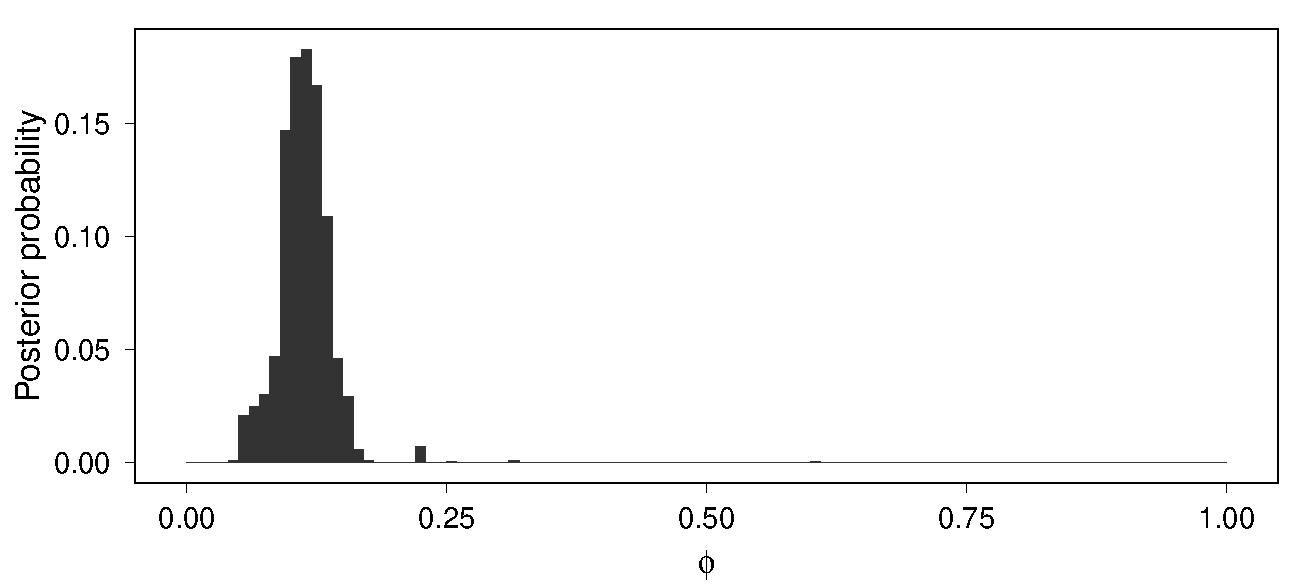
\includegraphics[width=0.8\columnwidth]{asym-phi-2opts-phi-100k.pdf}
    \caption{Posterior distribution of the contamination (``guessing'') parameter. The 95\% credible interval is [0.06, 0.15].}
  \label{fig:phi2}
\end{figure}

The estimated posterior distribution of the speaker rationality parameters $\lambda_{\text{truth conditions}}$ and $\lambda_{\text{implied prevalence}}$ are shown in Figure \ref{fig:rationality2}. 
This parameter represents the belief in how rational the hypothetical speaker in Eq.~{ref:eqS1} is believed to be when choosing to say the generic (over saying nothing). 
The 95\% credible interval for $\lambda_{\text{truth conditions}}$ is [0.23, 6.9] and $\lambda_{\text{implied prevalence}}$ is [1.30, 16.86]. The fact that these parameters are so different is expected given that the state space in the two tasks is also quite different.


\begin{figure}
\centering
    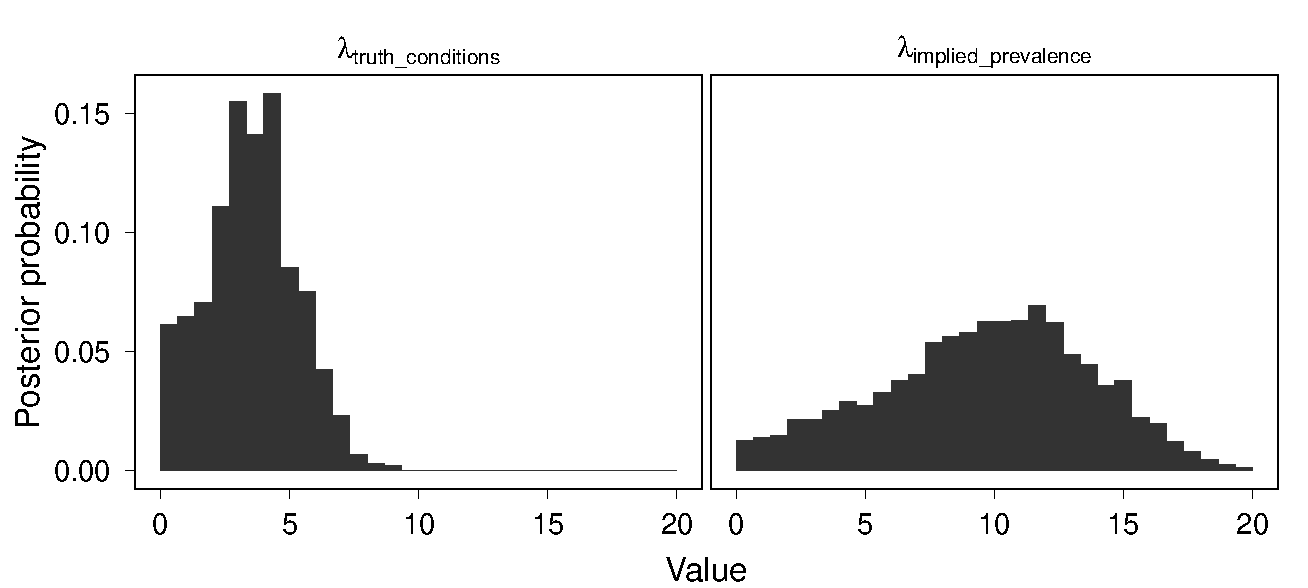
\includegraphics[width=0.8\columnwidth]{asym-lambdas-2opts-phi-100k.pdf}
    \caption{Posterior distribution of the speaker rationality parameters. The 95\% credible interval for $\lambda_{\text{truth conditions}}$ is [0.23, 6.9] and  $\lambda_{\text{implied prevalence}}$ is [1.30, 16.86]. The fact that these parameters are so different is expected given that the state space in the two tasks is also quite different.}
  \label{fig:rationality2}
\end{figure}




\section{General discussion}

The lifted-threshold RSA model presented in this paper takes a generic statement to be vague. ``K has F'' means ``many members of K have F, \emph{relative to other categories, the vast majority of which, very few or none of the individuals in those categories have F}''. 
The model predicts a range of truth judgments for generics that seem to not have to do with prevalence. 
By considering not only the prevalence within the category but prevalence across categories, the model is able to arrive at graded and property-sensitive predictions about the truth judgments of generic statements, as seen in Expt.~1. 
The model very naturally accounts for the parallel problem of generic interpretation. 
Different \emph{a priori} beliefs about the distributions of properties both within- and across-categories give rise the puzzling asymmetries in how generics are interpreted relative to what is needed to felicitously use the generic. 

We present a context-invariant semantics for generic statements. 
The stable meaning of a generic is as simple as possible: a threshold on prevalence, where the threshold is uncertain \emph{a priori} and only resolved by pragmatic reasoning.
This simple semantics is consistent with the profound phenomenon from cognitive development: Generics are learned at a very young age \cite{Gelman1998, Gelman2004, Gelman2008, Cimpian2008}.

We have explained two outstanding puzzles in language understanding. 
The first is that generic utterances can be true for a wide range of prevalence levels: from tigers with stripes all the way down to mosquitos with West Nile Virus. 
How can the prevalence of the property alone explain what makes some generics good things to say and others not as good? 
The insight is that with an uncertain semantics, the likely meaning of the generic (i.e. the likely threshold for acceptance) is inferred using listeners' \emph{a priori} beliefs and the communicative force of a speech act. 
This leads to different thresholds for different types of properties. 

The second phenomenon is the generic utterances often carry strong implications, though not all bare plurals have this impact. 
We measured participants' beliefs about the distributions of properties and found the accidental properties are utterly distinct in shape from biological properties.
Biological properties are characterized by \emph{widespread prevalence}, even though they may be rare across kinds (e.g. purple feathers).
Accidental properties, by contrast, are both rare across and within kinds: \emph{broken legs} are \emph{a priori} most likely to present in a small fraction of the population.
Thus, when given a vague utterance in the form a generic, the most likely \emph{a posteriori} prevalences vary in ways that match human participants' intuitions about the implied prevalence.


\subsection{Conceptual distinctions and prevalence}

We have shown that the truth conditions and implications of generics can be explained by beliefs about the prevalence of properties within- and across- categories. 
However, there is an open question of where \emph{these distributions} come from. 
It is quite plausible that these distributions are derived from higher-order conceptual knowledge about the nature of these properties \cite{Gelman2005, Keil1992}.

In Expt.~1a, participants estimated the prevalence of properties for many different kinds of animals. This was aggregated to form a distribution of prevalence across kinds.
In Expt.~2a, we measured this distribution by sequentially asking questions at different levels of abstraction: Question 1 was about the prevalence across categories while Question 2 was about prevalence within categories. 
It is likely that further abstracting the problem to more conceptual level questions (e.g. ``Are there differences between male and female lorches?''; ``Do you think a young fep is likely to have long legs?'') would elucidate the connection between distributions on prevalence and conceptual representations. 

Much of the psychological and philosophical work has looked beyond prevalence and focused on conceptual distinctions among generics \cite{Prasada2013, Leslie2008}. For example, \citeauthor{Prasada2013} has argued for a distinction between \emph{characteristic} properties (e.g. ``Diapers are absorbent.'') and \emph{statistical} properties (e.g. ``Diapers are white.''). Where in the prevalence-based semantics could such conceptual distinctions come into play?

Probabilistic models are a useful way to represent rich, structured knowledge of world \cite{Goodmanconcepts}. It's plausible that the prevalence distribution we've focused on in this work is actually derived from richer conceptual knowledge. For the purpose of the semantics of generics, this work shows that prevalence is sufficient to capture the range of truth judgments for these sentences. How a listener arrives at an estimate of the prevalence, or the prevalence distribution at large, may be the result of a probabilistic, conceptual model of the world. 

It's important to stress that our approach puts at its core listeners' \emph{beliefs} about the prevalence of the properties in question. 
Our participants' estimated the prevalence of certain properties to be much higher than the actual statistics of the world \red(example?).
This is an important methodological contrast to what is often employed in semantic approaches to generics, that prevalence is about \emph{actual prevalence in the world}. 
Along similar lines, this work used utterances about animal kinds in these experiments because participants' beliefs about these properties and categories are likely to be relatively homogenous (thus, lower noise). However, generic language is often used in everyday conversation to talk about social categories: In these domains, we would expect large individual differences in generic acceptability and interpretations.


An additional issue, one that likely interacts with conceptual distinctions, is how to determine the kinds of things against which a speaker implicitly compares the prevalence of the category in question. Here, we have used only generic sentences about animals, where the likely contrast class is other animals (e.g. ``Mosquitos carry malaria, \emph{relative to other kinds of living creatures}''). Moving outside the domain of animals, the makeup of this contrast class becomes less clear. 


A further observation concerning the nature of this contrast class is that focus, as a result of prosodic cues for example, can change the distribution against which one compares the prevalence of a property. For example, is a person asks ``What carries malaria?'', a very natural answer would be ``MOSQUITOS carry malaria'', since Mosquitos more than any other animal kind carry malaria. By contrast, if a person asks ``What are mosquitos like?'', is it natural to reply ``Mosquitos CARRY MALARIA''? 
Our suspicion is that it is not as natural because of salient alternatives (``Mosquitos bite you'', ``Mosquitos suck blood.'', ``Mosquitos make buzzing sounds''). 
Here, the contrast class is not with respect to \emph{other animals} but with respect to other properties \emph{of that animal}. 
Notice, however, that the underlying dimension that these properties would be compared along is still prevalence. What has changed is what constitutes this distribution: prevalence across categories vs. prevalence across properties.

\subsection{Resilience to counter-examples}

Another main staple of generic utterances is that they are resilient to counter-examples. 
For example, observing a few (perhaps, well-behaved) dogs that do not bark does not falsify ``Dogs bark.'' 
If generic statements are indeed vague, this phenomenon is very similar to the Sorites' Paradox, wherein a vague utterance and a plausible inductive premise can lead to unintuitive conclusions.

To see the similarity, consider the Sorites Paradox for ``The Empire State Building is tall.'' The paradox comes out when the following argument is considered:

\begin{quotation}

The Empire State Building is tall.

Any building 0.5 meters shorter than a tall building is still tall.

Therefore, a single-story building is tall.

\end{quotation} 

The first premise is true with a high probability. 
The second premise, is true with high probability but becomes less plausible the shorter in height one's reference gets. 

For generics, the version of the Sorites would look like

\begin{quotation}
Dogs bark. 

If we observe one dog that doesn't bark, then we could still say ``Dogs bark''. 

Therefore, if there were no dogs that barked, we would still conclude ``Dogs bark''.
\end{quotation} 

One thing to notice is that generics' resilience to counter-examples bears a strong similarity to the traditional inductive premise of the Sorites. 
It may be that the this feature of generics falls out of the inherent uncertainty of the meaning (i.e. its vagueness).

It's also interesting to consider the conclusion of this generic Sorites. 
This takes a very similar form of classic thought-experiments in the linguistics literature (e.g. ``Even t.



\subsection{What are generics?}

Intuitions about what qualifies as a generic statement have led to the consensus that there are generic and non-generic meanings that can be derived from similar syntactic forms. For example,
\begin{quotation}
	(1) Tigers are massive. 
	
	(2) Tigers are on the front lawn.
\end{quotation}

Classically, (1) is understood as referring to the kind whereas (2) is understood as referring to a plurality of instances. 

In our follow-up to \citeauthor{Cimpian2010}'s study on the implied prevalence of generic statements about accidental properties, we found a gradient of implied prevalence, which was driven by listener's \emph{a priori} beliefs about the prevalence of the property. 
The finding that different properties receive variable interpretations suggests a categorical distinction between generic and non-generic bare plurals may not be necessary. 
Consider the following 

\begin{quotation}
	(3) Tigers are on front lawns. 
	
	(4) Tigers are in zoos.
	
	(5) Tigers are in open grasslands.
\end{quotation}

Many would argue that (3) is not generic. At the same time, it does seem to implicate more tigers than (2). The same can be observed by comparing (4) to (3). Indeed, (5) has the intuitive appeal of applying to a large chunk of the category. (5) could be interpreted generically. 

It seems that as you go from (3) - (5), the likely implied prevalence also increases, to the point where (5) might apply to category as a whole. 
With a generic whose meaning is vague, as we propose here, listeners need not make categorical distinctions to interpret a sentence. 
Rather, they only need consult their beliefs about the properties in question to resolve reasonable interpretations. 

\subsection{Vagueness and communication}

We have presented a semantics for generics in which they convey a threshold on prevalence which is uncertain but fixed through pragmatic reasoning about the distribution of prevalence for the property in question.
In Expt.~2a, we showed how this prevalence distribution can be elicited by sequentially asking about the prevalence across- and within- categories. 
Within-category prevalence was elicited by asking a question about generalization: ``Imagine there is a glippet that has green legs. What \% of glippets do you think have green legs?''.

The model of generic communication that we've introduced uses a threshold whose value is uncertain. 
In a sense, the bare minimum that the generic communicates is that we are in a situation where there is a glippet that has green legs. 
The listener then is then left to her own devices to generalize as widely as she deems based on her beliefs about the property. 
This is consistent with the notion of a GEN operator that tells the listener to generalize this fact \cite{Leslie2008}.


The generic, it seems, doesn't convey any additional information beyond what the listener already knew about the prevalence of the property.
This shouldn't surprise us. ``John is tall'' does not actually tell us about what \emph{tall} means\footnote{However, ``John is a person'' does tell a listener about what \emph{tall} means in ``John is tall''.}. 
Rather, the listener is expected to come to the conversation with some beliefs about heights, and knowing that John is a person, be able to infer likely meanings for \emph{tall}.


\subsection{Conclusion} 


We have explored and demonstrated the viability of a scalar semantics for generics when coupled with a sophisticated pragmatics. 
A lower-bound threshold on prevalence---the probability of the property given the category---is inferred as part of pragmatic interpretation, yielding vague and context sensitive meanings. 

We formalized reasoning about the threshold in a lifted-threshold Rational Speech Acts model. This model predicted graded truth judgements and an asymmetry between truth and prevalence judgments. It also naturally accommodates the role of context, explaining these effects as the result of variation in the prevalence prior. 

Generics are ubiquitous in natural language. It might seem paradoxical, then, that the semantics of generic statements are underspecified. Why should vague language get so much usage? One possibility is apparent in the lifted-variable RSA model: generic language provides interlocutors with the flexibility to convey meanings as rich as our conceptual knowledge. %, which are easily understood in context. 
Generics are vague, but predictable and useful.

